\documentclass[12pt,a4]{article}

\usepackage{graphicx}

\begin{document}

% GNUPLOT: LaTeX picture with Postscript
\begingroup
  \makeatletter
  \providecommand\color[2][]{%
    \GenericError{(gnuplot) \space\space\space\@spaces}{%
      Package color not loaded in conjunction with
      terminal option `colourtext'%
    }{See the gnuplot documentation for explanation.%
    }{Either use 'blacktext' in gnuplot or load the package
      color.sty in LaTeX.}%
    \renewcommand\color[2][]{}%
  }%
  \providecommand\includegraphics[2][]{%
    \GenericError{(gnuplot) \space\space\space\@spaces}{%
      Package graphicx or graphics not loaded%
    }{See the gnuplot documentation for explanation.%
    }{The gnuplot epslatex terminal needs graphicx.sty or graphics.sty.}%
    \renewcommand\includegraphics[2][]{}%
  }%
  \providecommand\rotatebox[2]{#2}%
  \@ifundefined{ifGPcolor}{%
    \newif\ifGPcolor
    \GPcolorfalse
  }{}%
  \@ifundefined{ifGPblacktext}{%
    \newif\ifGPblacktext
    \GPblacktexttrue
  }{}%
  % define a \g@addto@macro without @ in the name:
  \let\gplgaddtomacro\g@addto@macro
  % define empty templates for all commands taking text:
  \gdef\gplbacktext{}%
  \gdef\gplfronttext{}%
  \makeatother
  \ifGPblacktext
    % no textcolor at all
    \def\colorrgb#1{}%
    \def\colorgray#1{}%
  \else
    % gray or color?
    \ifGPcolor
      \def\colorrgb#1{\color[rgb]{#1}}%
      \def\colorgray#1{\color[gray]{#1}}%
      \expandafter\def\csname LTw\endcsname{\color{white}}%
      \expandafter\def\csname LTb\endcsname{\color{black}}%
      \expandafter\def\csname LTa\endcsname{\color{black}}%
      \expandafter\def\csname LT0\endcsname{\color[rgb]{1,0,0}}%
      \expandafter\def\csname LT1\endcsname{\color[rgb]{0,1,0}}%
      \expandafter\def\csname LT2\endcsname{\color[rgb]{0,0,1}}%
      \expandafter\def\csname LT3\endcsname{\color[rgb]{1,0,1}}%
      \expandafter\def\csname LT4\endcsname{\color[rgb]{0,1,1}}%
      \expandafter\def\csname LT5\endcsname{\color[rgb]{1,1,0}}%
      \expandafter\def\csname LT6\endcsname{\color[rgb]{0,0,0}}%
      \expandafter\def\csname LT7\endcsname{\color[rgb]{1,0.3,0}}%
      \expandafter\def\csname LT8\endcsname{\color[rgb]{0.5,0.5,0.5}}%
    \else
      % gray
      \def\colorrgb#1{\color{black}}%
      \def\colorgray#1{\color[gray]{#1}}%
      \expandafter\def\csname LTw\endcsname{\color{white}}%
      \expandafter\def\csname LTb\endcsname{\color{black}}%
      \expandafter\def\csname LTa\endcsname{\color{black}}%
      \expandafter\def\csname LT0\endcsname{\color{black}}%
      \expandafter\def\csname LT1\endcsname{\color{black}}%
      \expandafter\def\csname LT2\endcsname{\color{black}}%
      \expandafter\def\csname LT3\endcsname{\color{black}}%
      \expandafter\def\csname LT4\endcsname{\color{black}}%
      \expandafter\def\csname LT5\endcsname{\color{black}}%
      \expandafter\def\csname LT6\endcsname{\color{black}}%
      \expandafter\def\csname LT7\endcsname{\color{black}}%
      \expandafter\def\csname LT8\endcsname{\color{black}}%
    \fi
  \fi
  \setlength{\unitlength}{0.0500bp}%
  \begin{picture}(7200.00,5040.00)%
    \gplgaddtomacro\gplfronttext{%
      \csname LT0\endcsname%
      \put(264,4930){\makebox(0,0)[l]{\strut{}epslatex  terminal test}}%
      \csname LT3\endcsname%
      \put(2280,2520){\makebox(0,0)[l]{\strut{}12345678901234567890}}%
      \put(2280,2828){\makebox(0,0)[l]{\strut{}test of character width:}}%
      \csname LTb\endcsname%
      \put(3600,3840){\makebox(0,0)[l]{\strut{}left justified}}%
      \put(3600,3620){\makebox(0,0){\strut{}centre+d text}}%
      \put(3600,3400){\makebox(0,0)[r]{\strut{}right justified}}%
      \csname LT1\endcsname%
      \put(220,2520){\rotatebox{-270}{\makebox(0,0){\strut{}rotated ce+ntred text}}}%
      \put(660,2520){\rotatebox{45}{\makebox(0,0)[l]{\strut{} rotated by +45 deg}}}%
      \put(440,2520){\rotatebox{-45}{\makebox(0,0)[l]{\strut{} rotated by -45 deg}}}%
      \csname LT4\endcsname%
      \put(3468,4804){\makebox(0,0)[r]{\strut{}show ticscale}}%
      \csname LTb\endcsname%
      \put(6345,4820){\makebox(0,0)[r]{\strut{}-1}}%
      \csname LTa\endcsname%
      \put(6345,4600){\makebox(0,0)[r]{\strut{}0}}%
      \csname LT0\endcsname%
      \put(6345,4380){\makebox(0,0)[r]{\strut{}1}}%
      \csname LT1\endcsname%
      \put(6345,4160){\makebox(0,0)[r]{\strut{}2}}%
      \csname LT2\endcsname%
      \put(6345,3940){\makebox(0,0)[r]{\strut{}3}}%
      \csname LT3\endcsname%
      \put(6345,3720){\makebox(0,0)[r]{\strut{}4}}%
      \csname LT4\endcsname%
      \put(6345,3500){\makebox(0,0)[r]{\strut{}5}}%
      \csname LT5\endcsname%
      \put(6345,3280){\makebox(0,0)[r]{\strut{}6}}%
      \csname LT6\endcsname%
      \put(6345,3060){\makebox(0,0)[r]{\strut{}7}}%
      \csname LT7\endcsname%
      \put(6345,2840){\makebox(0,0)[r]{\strut{}8}}%
      \csname LT8\endcsname%
      \put(6345,2620){\makebox(0,0)[r]{\strut{}9}}%
      \csname LT0\endcsname%
      \put(6345,2400){\makebox(0,0)[r]{\strut{}10}}%
      \csname LT1\endcsname%
      \put(6345,2180){\makebox(0,0)[r]{\strut{}11}}%
      \csname LT2\endcsname%
      \put(6345,1960){\makebox(0,0)[r]{\strut{}12}}%
      \csname LT3\endcsname%
      \put(6345,1740){\makebox(0,0)[r]{\strut{}13}}%
      \csname LT4\endcsname%
      \put(6345,1520){\makebox(0,0)[r]{\strut{}14}}%
      \csname LT5\endcsname%
      \put(6345,1300){\makebox(0,0)[r]{\strut{}15}}%
      \csname LT6\endcsname%
      \put(6345,1080){\makebox(0,0)[r]{\strut{}16}}%
      \csname LT7\endcsname%
      \put(6345,860){\makebox(0,0)[r]{\strut{}17}}%
      \csname LT8\endcsname%
      \put(6345,640){\makebox(0,0)[r]{\strut{}18}}%
      \csname LT0\endcsname%
      \put(6345,420){\makebox(0,0)[r]{\strut{}19}}%
      \csname LTb\endcsname%
      \put(1260,201){\makebox(0,0)[l]{\strut{}  lw 1}}%
      \put(1260,402){\makebox(0,0)[l]{\strut{}  lw 2}}%
      \put(1260,603){\makebox(0,0)[l]{\strut{}  lw 3}}%
      \put(1260,804){\makebox(0,0)[l]{\strut{}  lw 4}}%
      \put(1260,1005){\makebox(0,0)[l]{\strut{}  lw 5}}%
      \put(1260,1206){\makebox(0,0)[l]{\strut{}  lw 6}}%
      \put(540,1407){\makebox(0,0)[l]{\strut{}linewidth}}%
      \put(4860,960){\makebox(0,0){\strut{}pattern fill}}%
      \put(3690,740){\makebox(0,0){\strut{} 0}}%
      \put(3960,740){\makebox(0,0){\strut{} 1}}%
      \put(4230,740){\makebox(0,0){\strut{} 2}}%
      \put(4500,740){\makebox(0,0){\strut{} 3}}%
      \put(4770,740){\makebox(0,0){\strut{} 4}}%
      \put(5040,740){\makebox(0,0){\strut{} 5}}%
      \put(5310,740){\makebox(0,0){\strut{} 6}}%
      \put(5580,740){\makebox(0,0){\strut{} 7}}%
      \put(5850,740){\makebox(0,0){\strut{} 8}}%
      \put(6120,740){\makebox(0,0){\strut{} 9}}%
      \csname LTb\endcsname%
      \put(5040,4653){\makebox(0,0){\strut{}filled polygons:}}%
    }%
    \gplbacktext
    \put(0,0){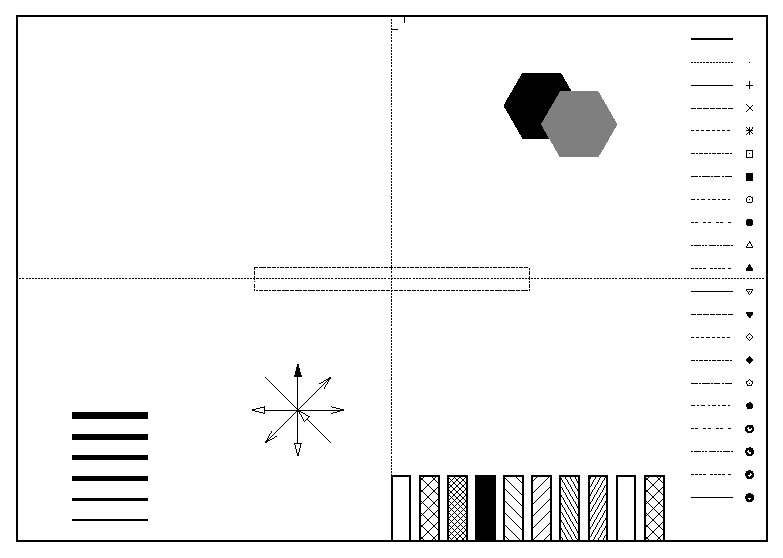
\includegraphics{test}}%
    \gplfronttext
  \end{picture}%
\endgroup

\end{document}
